\documentclass[twoside,10pt]{article}
\usepackage{/Users/bradenhoagland/latex/styles/toggles}
%\toggletrue{sectionbreaks}
%\toggletrue{sectionheaders}
\newcommand{\docTitle}{HW 3}
\usepackage{/Users/bradenhoagland/latex/styles/common}
\importStyles{modern}{rainbow}{boxy}

%\renewcommand{\theenumi}{\alph{enumi}}

\begin{document}
%\tableofcontents

% ------------------------------
% 1.2: 8
% ------------------------------
\begin{exer}[1.2: 8]
$\pi_1$ of two tori with coinciding circle.
\end{exer}

\begin{figure}[H]
	\centering
	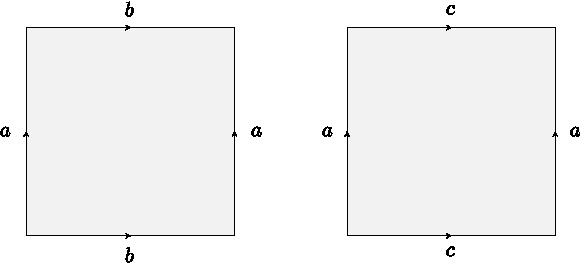
\includegraphics[scale=1]{fig/8.pdf}
	%\caption{}
\end{figure}

The situation is depicted above. We have two tori that share a common circle (in this case $a$). We fill these two 1-skeletons with 2-cells along the boundaries $aba^{-1}b^{-1}$ and $aca^{-1}c^{-1}$. Thus the fundamental group is
\[
	\ang{a,b,c \;|\; [a,b], [a,c]} \quad\cong\quad \mathbb{Z} \times (\mathbb{Z} * \mathbb{Z}).
\] 

\newpage

% ------------------------------
% 1.2: 9
% ------------------------------
\begin{exer}[1.2: 9]
$M_{g}$ doesn't retract to $C$, but it does retract to $C'$.
\end{exer}

\textbf{No retraction onto $C$:} Suppose $M_{h}'$ retracts onto $C$ via $r$, then since $\text{ab}$ is a covariant functor $\cat{Grp}\to \cat{Ab}$, we have the following sequence of induced maps.

\[
\begin{tikzcd}
	M_{h}' \dar[two heads, shift left]{r} & \pi_1(M_{h}') \dar[two heads, shift left]{r_{*}} & \text{ab}(\pi_1(M_{h}')) \dar[two heads, shift left]{\tilde{r}_{*}} \\
	C \uar[hook, shift left]{i} & \pi_1(C) \cong \mathbb{Z} \uar[hook, shift left]{i_{*}} & \mathbb{Z} \uar[hook, shift left]{\tilde{i}_{*}}
\end{tikzcd}
\] 

Functoriality of $\pi_1$ and $\text{ab}$ implies that $\tilde{r}_{*} \circ \tilde{i}_{*}=\id$; thus why the injectivity and surjectivity are preserved.

Now we have to derive a contradiction of some sort using these induced maps. We can depict $M_h'$ as below.

\begin{figure}[H]
	\centering
	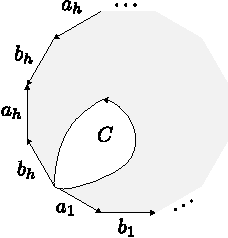
\includegraphics[scale=1]{fig/9a.pdf}
	%\caption{}
\end{figure}

From this figure, $C$ is clearly homotopic to $[a_1,b_1]\cdots [a_h,b_h]$, so $1 \in \pi_1(C) = \mathbb{Z}$ is mapped to $[a_1,b_1]\cdots [a_h,b_h] \in \pi(M_{h}')$ by $i_{*}$. But this is trivial once $\pi_1(M_{h}')$ is abelianized, so $\tilde{i}_{*}$ is a constant map, contradicting its injectivity. Thus $M_{h}'$ cannot retract onto $C$.

But if $M_{g}$ retracts onto $C$ via $r$, then $M_{h}'$ retracts onto $C$ via $r|_{M_{h}'}$, so this also implies that $M_{g}$ cannot retract onto $C$.

\textbf{Retraction onto $C'$:} The following image shows a retraction $M_{g} \to M_{1} = S^{1}\times S^{1}$. We can compose this with the projection map onto one coordinate of $S^{1}\times S^{1}$, giving a retraction onto $C'$.

\begin{figure}[H]
	\centering
	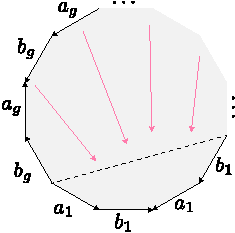
\includegraphics[scale=1]{fig/9b.pdf}
	%\caption{}
\end{figure}

\newpage

% ------------------------------
% 1.2: 11
% ------------------------------
\begin{exer}[1.2: 11]
	Mapping tori of $S_1 \vee S_1$ and $S_1 \times S_1$.
\end{exer}

\textbf{First part:} Suppose $x_0$ is the basepoint connecting the two circles in $X = S^{1}\vee S^{1}$, then since $f$ is basepoint-preserving, we get the following picture.

\begin{figure}[H]
	\centering
	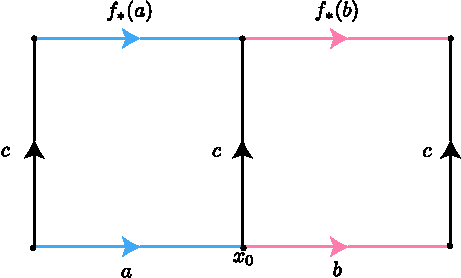
\includegraphics[scale=1]{fig/11a.pdf}
	%\caption{}
\end{figure}

Each of the 6 vertices is identified into one 0-cell, and there are three distinct lines (1-cells) going out of and into this point, so the 1-skeleton is $S^{1}\vee S^{1}\vee S^{1}$.

Then $T_{f}$ is then recovered from the 1-skeleton by gluing on 2-cells along $acf_{*}(a)^{-1}c^{-1}$ and $bcf_{*}(b)^{-1}c^{-1}$. Thus the fundamental group of $T_{f}$ is
\[
	\pi_1(T_{f}) = \ang{a,b,c \;|\; acf_{*}(a)^{-1}c^{-1},\; bcf_{*}(b)^{-1}c^{-1}}.
\] 

\textbf{Second part:} Suppose instead that $X = S' \times S'$, then the new 1-skeleton is pictured below.

\begin{figure}[H]
	\centering
	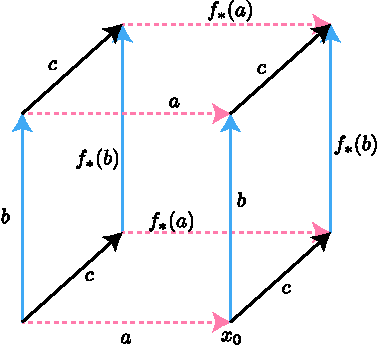
\includegraphics[scale=1]{fig/11b.pdf}
	%\caption{}
\end{figure}
Note that all of the 8 vertices are identified with $x_0$.

Note that since all the vertices are identified and since there are three distinct 1-cells, this is $S_1^{1} \vee S^{1}\vee S^{1}$. To fill it, attach three 2-cells along $aba^{-1}b, bcf_{*}(b)^{-1}c^{-1}$, and $acf_{*}(a)^{-1}c^{-1}$. Thus the fundamental group is
\[
	\pi_1(T_{f}) \cong \ang{a,b,c \;|\; [a,b], bcf_{*}(b)^{-1}c^{-1}, acf_{*}(a)^{-1}c^{-1}}.
\] 


\newpage

% ------------------------------
% 1.2: 14
% ------------------------------
\begin{exer}[1.2: 14]
Funky cube with $\pi_1$ the quaternion group.
\end{exer}

The 1-skeleton of this space is pictured below, with 1-cells of the same color and 0-cells of the same shape identified.

\begin{figure}[H]
	\centering
	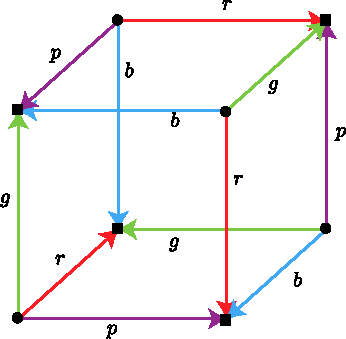
\includegraphics[scale=1]{fig/14.pdf}
	%\caption{}
\end{figure}

Because of the identifications, this is just $S^{1}\vee S^{1}\vee S^{1}$. I found that $pb^{-1}, pr^{-1},$ and $pg^{-1}$ generate all other loops by simply checking all cases. We can add in 2-cells along the right, back, and top faces to fill in the space. Thus the fundamental group is
\begin{align*}
	\pi_1(X) &\cong \ang{pb^{-1}, pr^{-1}, pg^{-1} \;|\; pg^{-1}rb^{-1}, pr^{-1}bg^{-1}, pb^{-1}gr^{-1}}.
	\intertext{Now we can define $i \doteq pb^{-1}, j \doteq pr^{-1}$, and $j \doteq pg^{-1}$, which makes this}
		 &= \ang{i,j,k \;|\; kj^{-1}i, ji^{-1}k, ik^{-1}j} \\
		 &= \ang{i,j,k \;|\; j=ki, i=jk, k=ij} \\
		 &= \ang{i,j,k \;|\; i^2=j^2=k^2=ijk}.
\end{align*}
This is exactly the quaternion group.

\newpage

\end{document}
